\RCS$Revision: 423381 $
\RCS$HeadURL: svn+ssh://svn.cern.ch/reps/tdr2/papers/HIN-16-011/trunk/HIN-16-011.tex $
\RCS$Id: HIN-16-011.tex 423381 2017-09-01 14:20:05Z alverson $
\newlength\cmsFigWidth
\ifthenelse{\boolean{cms@external}}{\setlength\cmsFigWidth{0.98\columnwidth}}{\setlength\cmsFigWidth{0.69\textwidth}}
\ifthenelse{\boolean{cms@external}}{\providecommand{\cmsLeft}{top\xspace}}{\providecommand{\cmsLeft}{left\xspace}}
\ifthenelse{\boolean{cms@external}}{\providecommand{\cmsRight}{bottom\xspace}}{\providecommand{\cmsRight}{right\xspace}}
\newcommand{\sqrts}{ \ensuremath{\sqrt{s}}\xspace}
\newcommand{\sqrtsNN}{ \ensuremath{\sqrt{\smash[b]{s_{_{\mathrm{NN}}}}}}\xspace}
\newcommand{\Bplusminusdecay}{\ensuremath{\PBpm\to\PJGy~\PKpm\to\Pgmp\Pgmm\PKpm}\xspace}
\newcommand{\Bjpsixdecay}{\ensuremath{\PB\to\PJGy~\cmsSymbolFace{X}}\xspace}
\newcommand{\RAA}{\ensuremath{R_{\mathrm{AA}}}\xspace}
\newcommand{\TAA}{\ensuremath{T_{\mathrm{AA}}}\xspace}
\newcommand{\pPb}{\ensuremath{\Pp\mathrm{Pb}}\xspace}
\newcommand{\PbPb}{\ensuremath{\mathrm{PbPb}}\xspace}
\newcommand{\Pb}{\ensuremath{\mathrm{Pb}}\xspace}
\newcommand{\pp}{\Pp\Pp\xspace}
\providecommand{\PBzeros}{\ensuremath{{\mathrm{B}_{s}^{0}}}}
\providecommand{\Pphi}{\ensuremath{\phi}}
\providecommand{\PDsp}{\ensuremath{\mathrm{D_{s}^{+}}}}
\providecommand{\Bzerosdecay}{\ensuremath{\PBzeros\to\PJGy~\Pphi\to\Pgmp\Pgmm\PKp\PKp}\xspace}
\providecommand{\mbinv} {\mbox{\ensuremath{\,\text{mb}^\text{$-$1}}}\xspace}
\providecommand{\HYDJET}{\textsc{hydjet}\xspace}

\cmsNoteHeader{HIN-16-011}

\title{\texorpdfstring{Measurement of the $\PBzeros$ meson nuclear modification factor in \PbPb collisions at $\sqrtsNN=5.02\TeV$}{Measurement of Bs+/- mesons nuclear modification factor in PbPb collisions at sqrt(s[NN]) = 5.02 TeV}}

\address[cern]{CERN}
\author[cern]{The CMS Collaboration}

\date{\today}

\abstract{
The differential production cross sections of $\PBzeros$ mesons and charge conjugates are measured via the exclusive decay channels \Bzerosdecay 
as a function of transverse momentum in \pp and \PbPb collisions at a center-of-mass energy $\sqrtsNN=5.02\TeV$ per nucleon pair with the CMS detector at the LHC.
The \pp (\PbPb) dataset used for this analysis corresponds to an integrated luminosity of 28.0\pbinv (351\mubinv).
The measurement is performed in the $\PBzeros$ meson transverse momentum range of 15 to 50\GeVc, in the rapidity interval $\abs{y}<2.4$. 
In this kinematic range, a strong suppression of the production cross section of $\PBzeros$ mesons by about a factor of two is observed in the \PbPb system in comparison 
to the expectation from \pp reference data. This result is found to be compatible with the one measured for the $\PBpm$ mesons at the same energy and rapidity. 
}

\hypersetup{%
pdfauthor={Ta-Wei Wang, Andrew Turner, Jing Wang, Dozen Candan, Kisoo Lee, Gian Michele Innocenti, Hyunchul Kim, Camelia Mironov, Yen-Jie Lee},%
pdftitle={Measurement of Bs+/- meson differential production cross sections in pp and PbPb collisions at sqrt(s[NN]) = 5.02 TeV},%
pdfsubject={CMS},%
pdfkeywords={physics, dimuons, proton Lead, charmonia, suppression, quark gluon plasma, shadowing, B meson, open heavy-flavor}}

\maketitle

Relativistic heavy ion collisions allow the study of quantum chromodynamics (QCD) at high energy density and temperature. Under such extreme conditions, a state consisting of deconfined 
quarks and gluons, the quark-gluon plasma (QGP)~\cite{QGP1,QGP2}, is predicted by lattice QCD calculations~\cite{Karsch:2003jg}. Heavy-quarks are effective probes to study the 
properties of this medium. Charm and beauty quarks, which are produced in hard scatterings at the early stages of the collision, are expected to lose energy via elastic collisions and 
medium-induced gluon radiation. The study of this phenomenon, called jet quenching~\cite{Eloss1,Baier:2000mf,Chatrchyan:2011sx,Aad:2010bu}, can provide strong insights into the 
energy density and diffusion properties of the Quark-Gluon Plasma.  The measurement of the suppression of strange beauty particles in heavy-ion collisions is 
also considered of fundamental importance to study the mechanisms of beauty hadronisation in heavy ion collisions. In presence of a medium with increased strangeness content 
as the QGP~\cite{ABELEV:2013zaa}, the relative yield of $\PBzeros$ mesons with respect to non-strange beauty mesons at low-intermediate \pt can be enhanced in nucleus-nucleus 
collisions as compared to pp interactions if recombination is a relevant mechanism of beauty hadronisation in the QGP~\cite{Molnar:2003ff,Greco:2003mm,Greco:2003vf}. 
An indication of the relevance of recombination, which is considered one of the golden probe to identify the presence of a deconfined medium, was recently observed in the charm sector by the ALICE 
Collaboration that measured an enhancement in the relative yield of $\PDsp$ mesons with respect to non-strange charmed mesons in central PbPb collisions at $\sqrts=5.02\TeV$~\cite{Adam2016Ds}.

The production of $\PBzeros$ mesons was measured at the LHC in pp collisions at center-of-mass energies of $\sqrts=7\TeV$~\cite{Chatrchyan:2011vh}
and in in proton-lead (pPb) collisions at a center-of-mass energy per nucleon pair $\sqrts=5.02\TeV$~\cite{Khachatryan:2015uja}.
In this Letter, we perform the first measurement of exclusive $\PBzeros$ mesons decays in PbPb collisions. The nuclear modification factor \RAA of $\PBp$ mesons, 
which is defined as the ratio of the cross section in PbPb collisions with respect to that in pp collisions scaled by the number of binary nucleon-nucleon (NN) collisions, 
is also presented. The comparison between the \RAA of $\PBzeros$ and the one of $\PBp$ mesons, which was also recently measured by the CMS Collaboration~\cite{PhysRevLett.119.152301}, provides
important insights into the role of beauty recombination in heavy-ion collisions. 


The $\PBzeros$ mesons and charge conjugates are measured at central rapidity ($\abs{y}<2.4$) via the reconstruction of the decay channels \Bzerosdecay, 
which have the branching fraction $\mathcal{B} = (3.12 \pm 0.24) \times 10^{-5}$~\cite{pdg:2016}.  The measurement is performed in pp collisions in four 
\pt bins ($[10,15]$, $[15,20]$, $[20,30]$, $[30,50]$\GeVc) and in one single \pt interval in PbPb collisions ($[10,50]$\GeVc). Throughout the paper, 
unless otherwise specified, the $y$ and \pt variables given are those of the $\PBzeros$ mesons. This analysis does not distinguish between the charge conjugates.


The central feature of the CMS detector is a superconducting solenoid which provides a magnetic field of 3.8\unit{T}. Within the solenoid volume are a silicon tracker which measures charged particles within the pseudorapidity range $\abs{\eta} < 2.5$, a lead tungstate crystal electromagnetic calorimeter, and a brass and scintillator hadron calorimeter. For typical particles of $1 < \pt < 10$\GeVc and $\abs{\eta} < 1.4$, the track resolutions are typically 1.5\% in \pt and 25--90 (45--150)\mum in the transverse (longitudinal) impact parameter \cite{TRK-11-001}. Muons are measured in the range $\abs{\eta} < 2.4$, with detection planes made using three technologies: drift tubes, cathode strip chambers, and resistive-plate chambers. The muon reconstruction algorithm starts by finding tracks in the muon detectors, which are then fitted together with tracks reconstructed in the silicon tracker to form "global muons". Matching muons to tracks measured in the silicon tracker results in a relative \pt resolution for muons with $20 < \pt < 100$\GeVc of 1.3--2.0\% in the barrel ($\abs{\eta} < 1.2$) and better than 6\% in the endcaps ($1.6 < \abs{\eta} < 2.4$).
For muons with higher \pt up to 1\TeVc, the \pt resolution in the barrel is better than 10\%~\cite{Chatrchyan:2012xi}.  The hadron forward (HF) calorimeter uses steel as an absorber and quartz fibers as the sensitive material. The two halves of the HF are located 11.2\unit{m} away from the interaction point, one on each end, providing together coverage in the range $3.0 < \abs{\eta} < 5.2$. In this analysis, the HF information is used for performing an offline event selection. A detailed description of the CMS experiment and coordinate system can be found in Ref.~\cite{bib_CMS}.

Several Monte Carlo (MC) simulated event samples are used to evaluate background components, signal efficiencies and detector acceptance corrections. This includes samples containing only the $\PBzeros$ mesons decays channels being measured, and samples with inclusive (prompt and nonprompt) $\PJGy$ mesons.
Proton-proton collisions are generated with \PYTHIA 8~\cite{Sjostrand:2014zea} tune CUETP8M1~\cite{Khachatryan:2015pea} and propagated through the CMS detector using the \GEANTfour package~\cite{geant4}.
The decay of the $\PBzeros$~mesons is modeled with the \EVTGEN 1.3.0~\cite{evtgen}, and final-state photon radiation in the $\PBzeros$ decays is simulated with \PHOTOS 2.0~\cite{Barberio:1990ms}. For the $\PbPb$ MC samples, each \PYTHIA 8 event is embedded into a $\PbPb$ collision event generated with {\HYDJET}~1.8~\cite{Lokhtin:2005px}, which is tuned to reproduce global event properties, such as the charged-hadron \pt spectrum and particle multiplicity.

Events were collected with the same trigger during the \pp and \PbPb data taking, requiring the presence of two muon candidates, with no explicit momentum threshold. For the offline analysis, events have to pass a set of selection criteria designed to reject events from background processes
(beam-gas collisions and beam scraping events) as described in Ref.~\cite{Khachatryan:2016odn}. Events are required to have
at least one reconstructed primary interaction vertex with a distance from the center of the nominal interaction region of less than 15\cm along the beam axis. In \PbPb collisions, the
shapes of the clusters in the pixel detector have to be compatible with those expected from particles produced by a \PbPb collision~\cite{Khachatryan:2010xs}. The \PbPb collision event is also required to have at least
three towers in each of the HF detectors with energy deposits of more than 3\GeV per tower. These criteria select $(99\pm2)$\% of inelastic hadronic \PbPb collisions. Selection efficiencies higher
than 100\% are possible, reflecting the possible presence of ultra-peripheral (i.e. nonhadronic) collisions in the selected event sample. The \PbPb sample corresponds to an integrated luminosity of approximately 351\mubinv. 
This value is indicative only, as the \PbPb yield is normalized by the total number of minimum-bias events sampled, $N_{\text{MB}}$. The \pp data set corresponds to an integrated luminosity of 28.0\pbinv, which is known to an accuracy of 2.3\% from the uncertainty in the calibration based on a van der Meer scan~\cite{CMS-PAS-LUM-16-001}.


\begin{figure*}[tb]
\centering
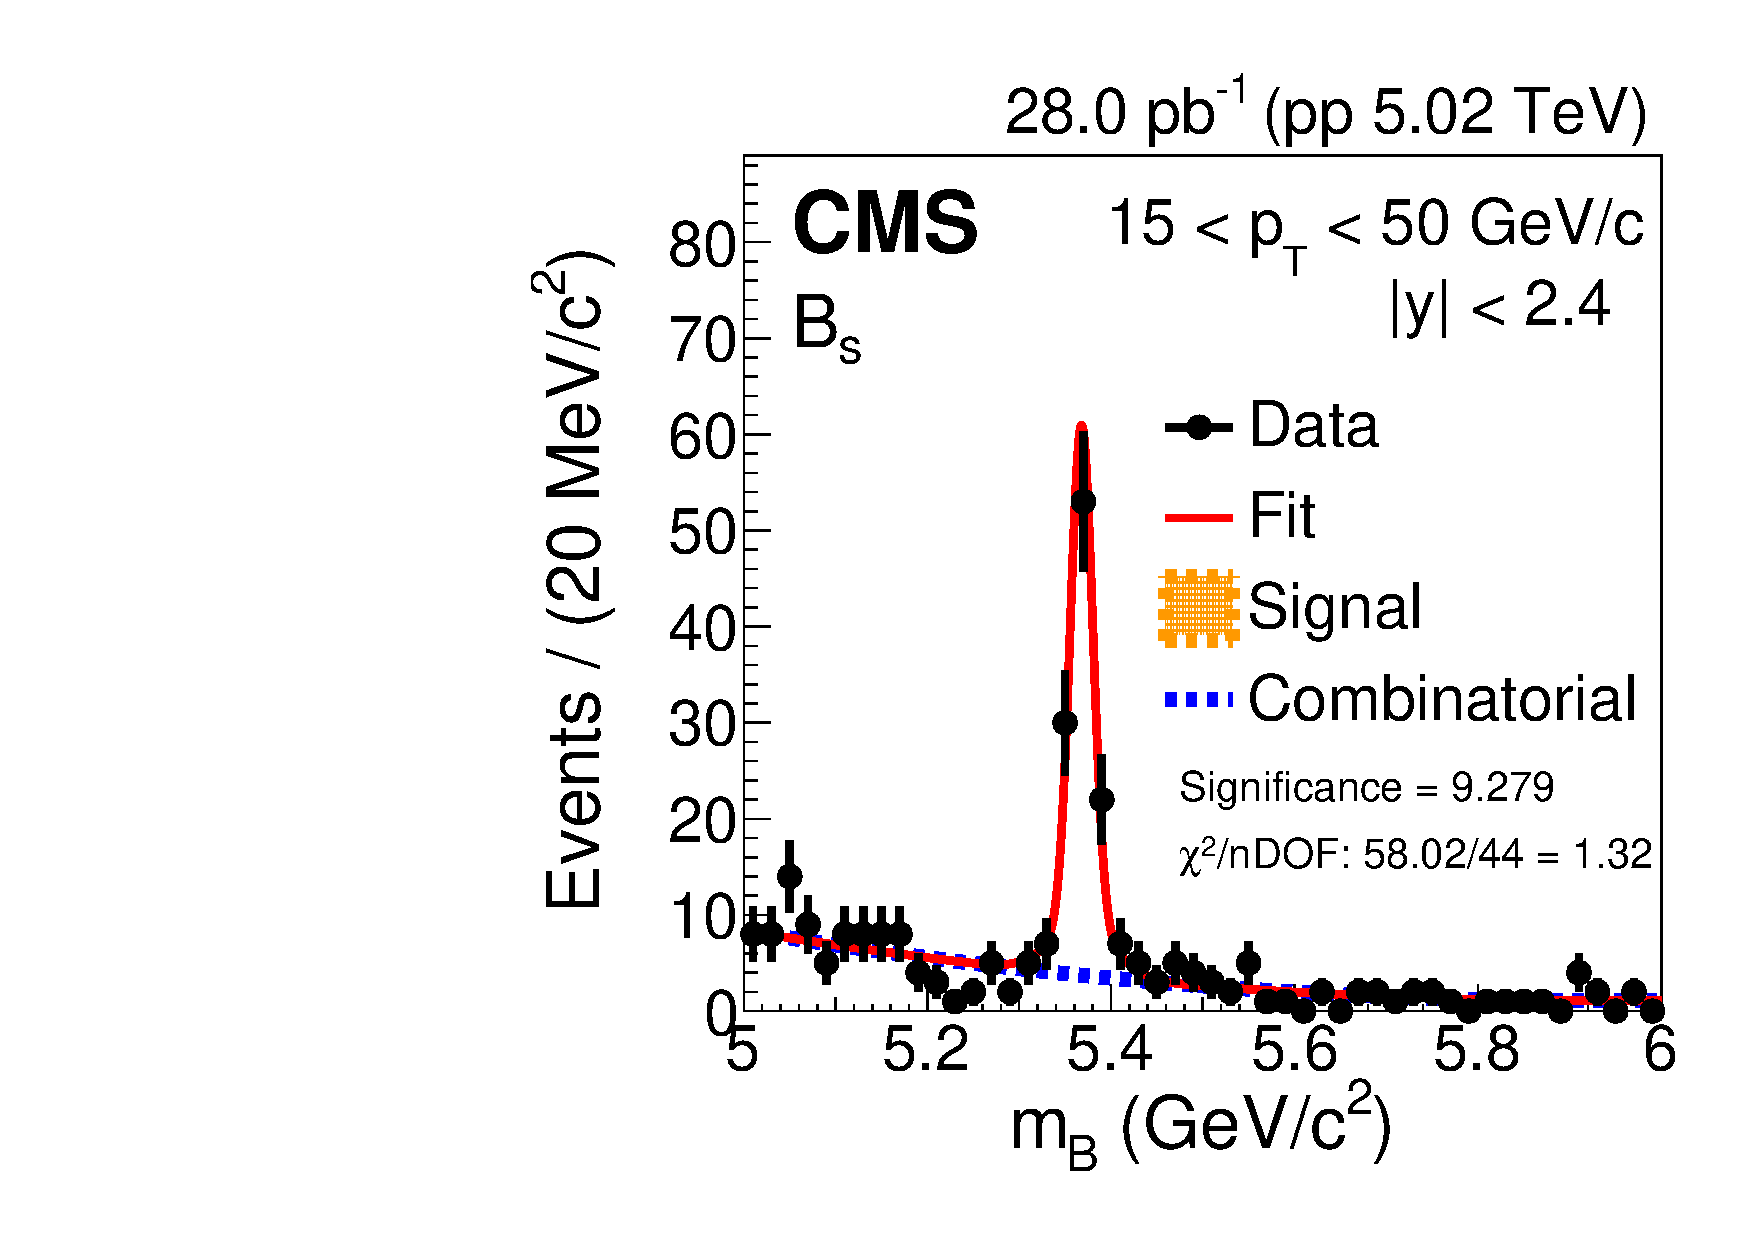
\includegraphics[width=.49\textwidth]{plots/data_pp_15_50.pdf}
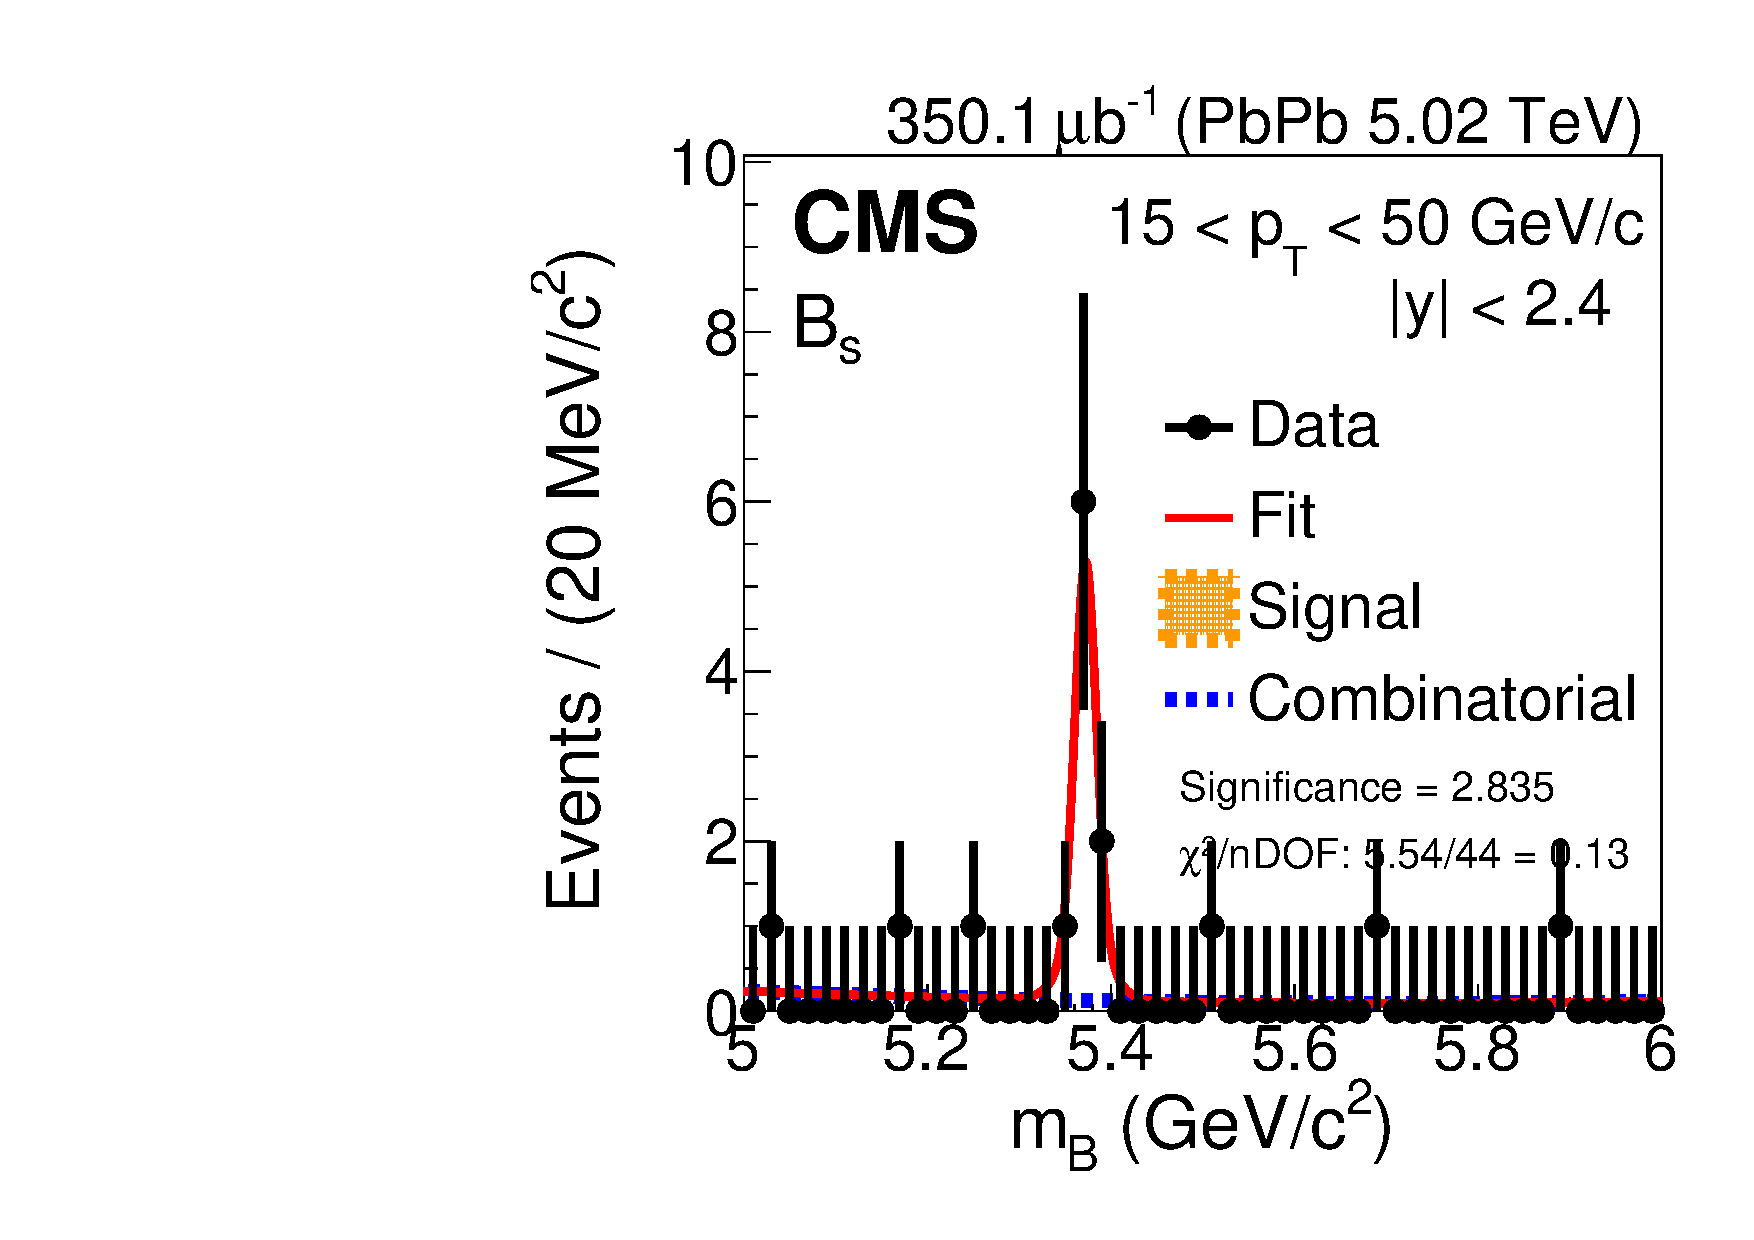
\includegraphics[width=.49\textwidth]{plots/data_PbPb_15_50.pdf}
\caption{Invariant mass distributions of $\PBzeros$ candidates in \pp (left) and \PbPb (right) collisions measured in $\abs{y}<2.4$ and in the \pt region 15--50\GeVc.} 
\label{fig:rawYieldsBsmeson}
\end{figure*}

\begin{figure*}[tb]
\centering
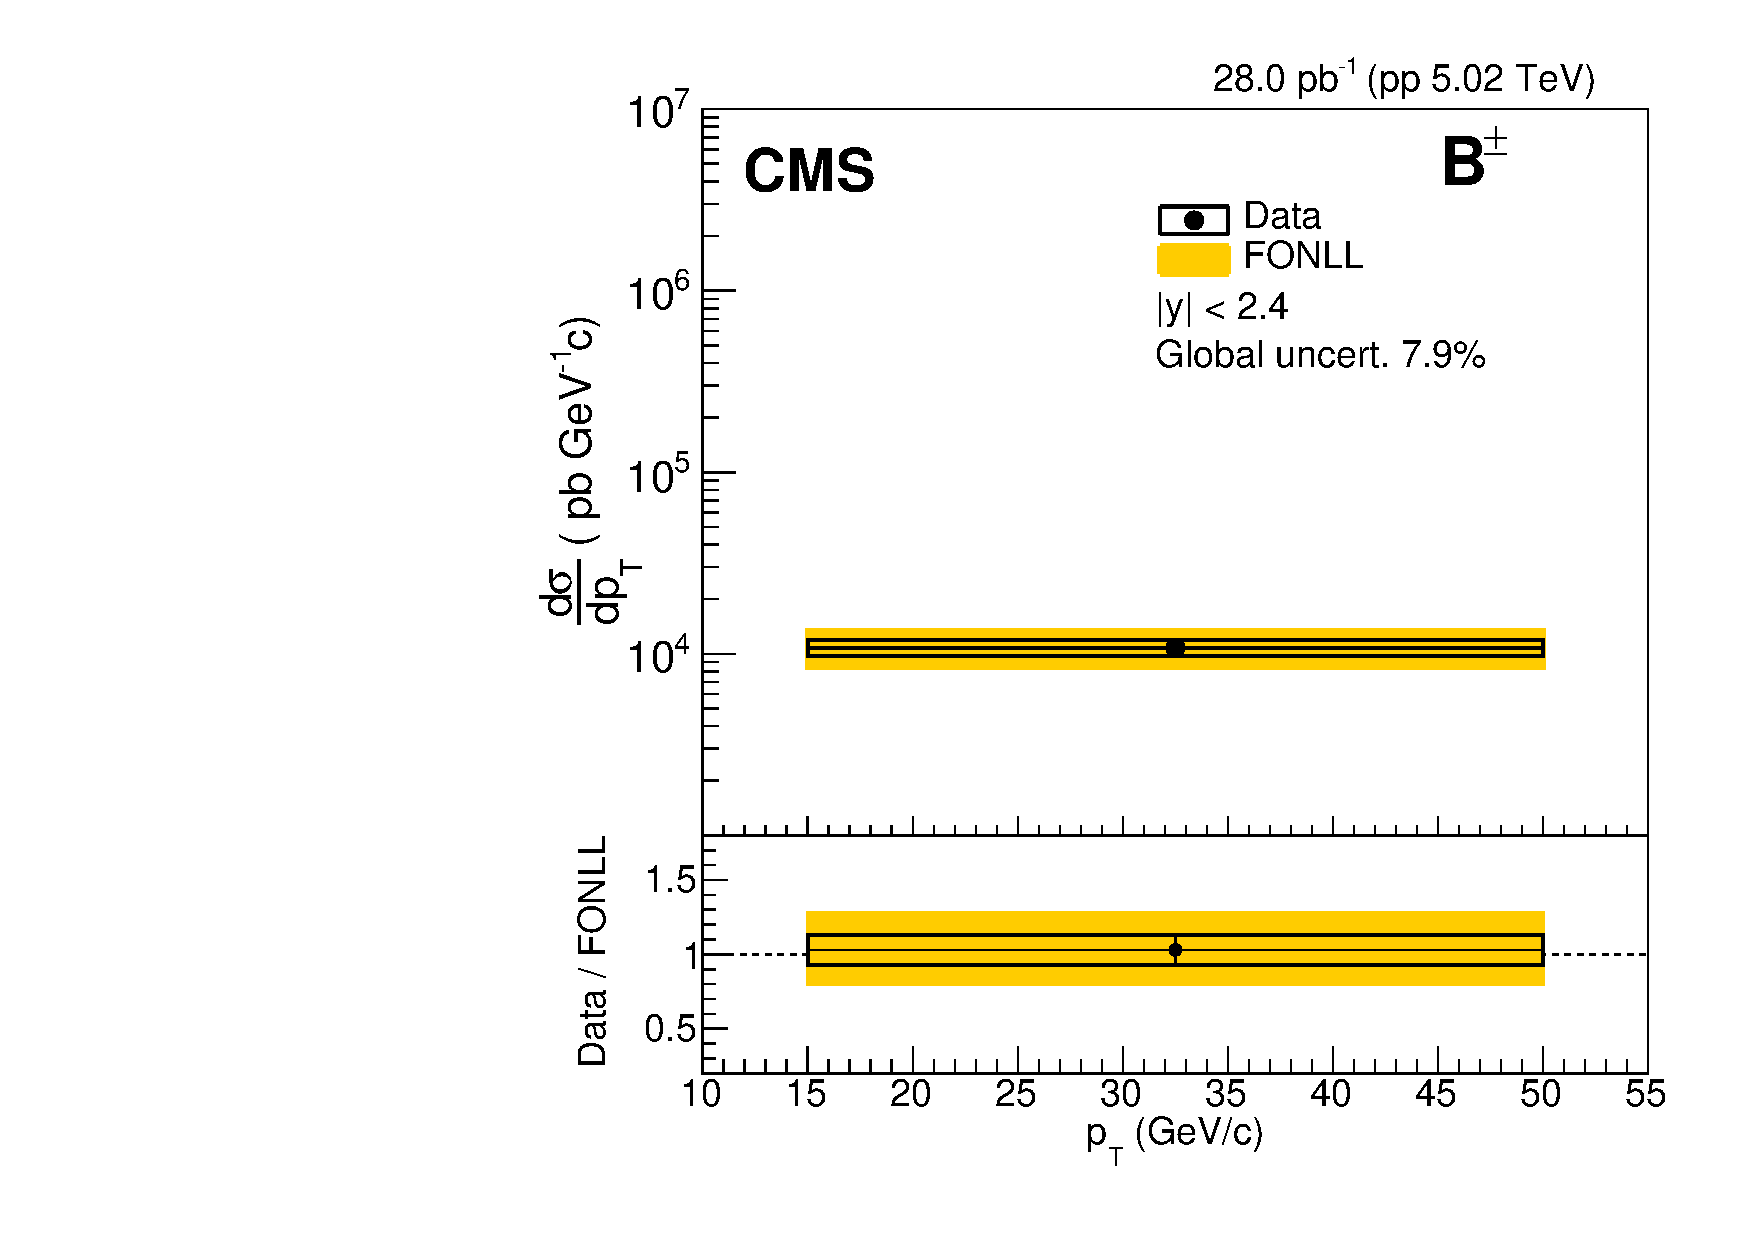
\includegraphics[width=.45\textwidth]{plots/canvasSigmaBplusRatiopp.pdf}
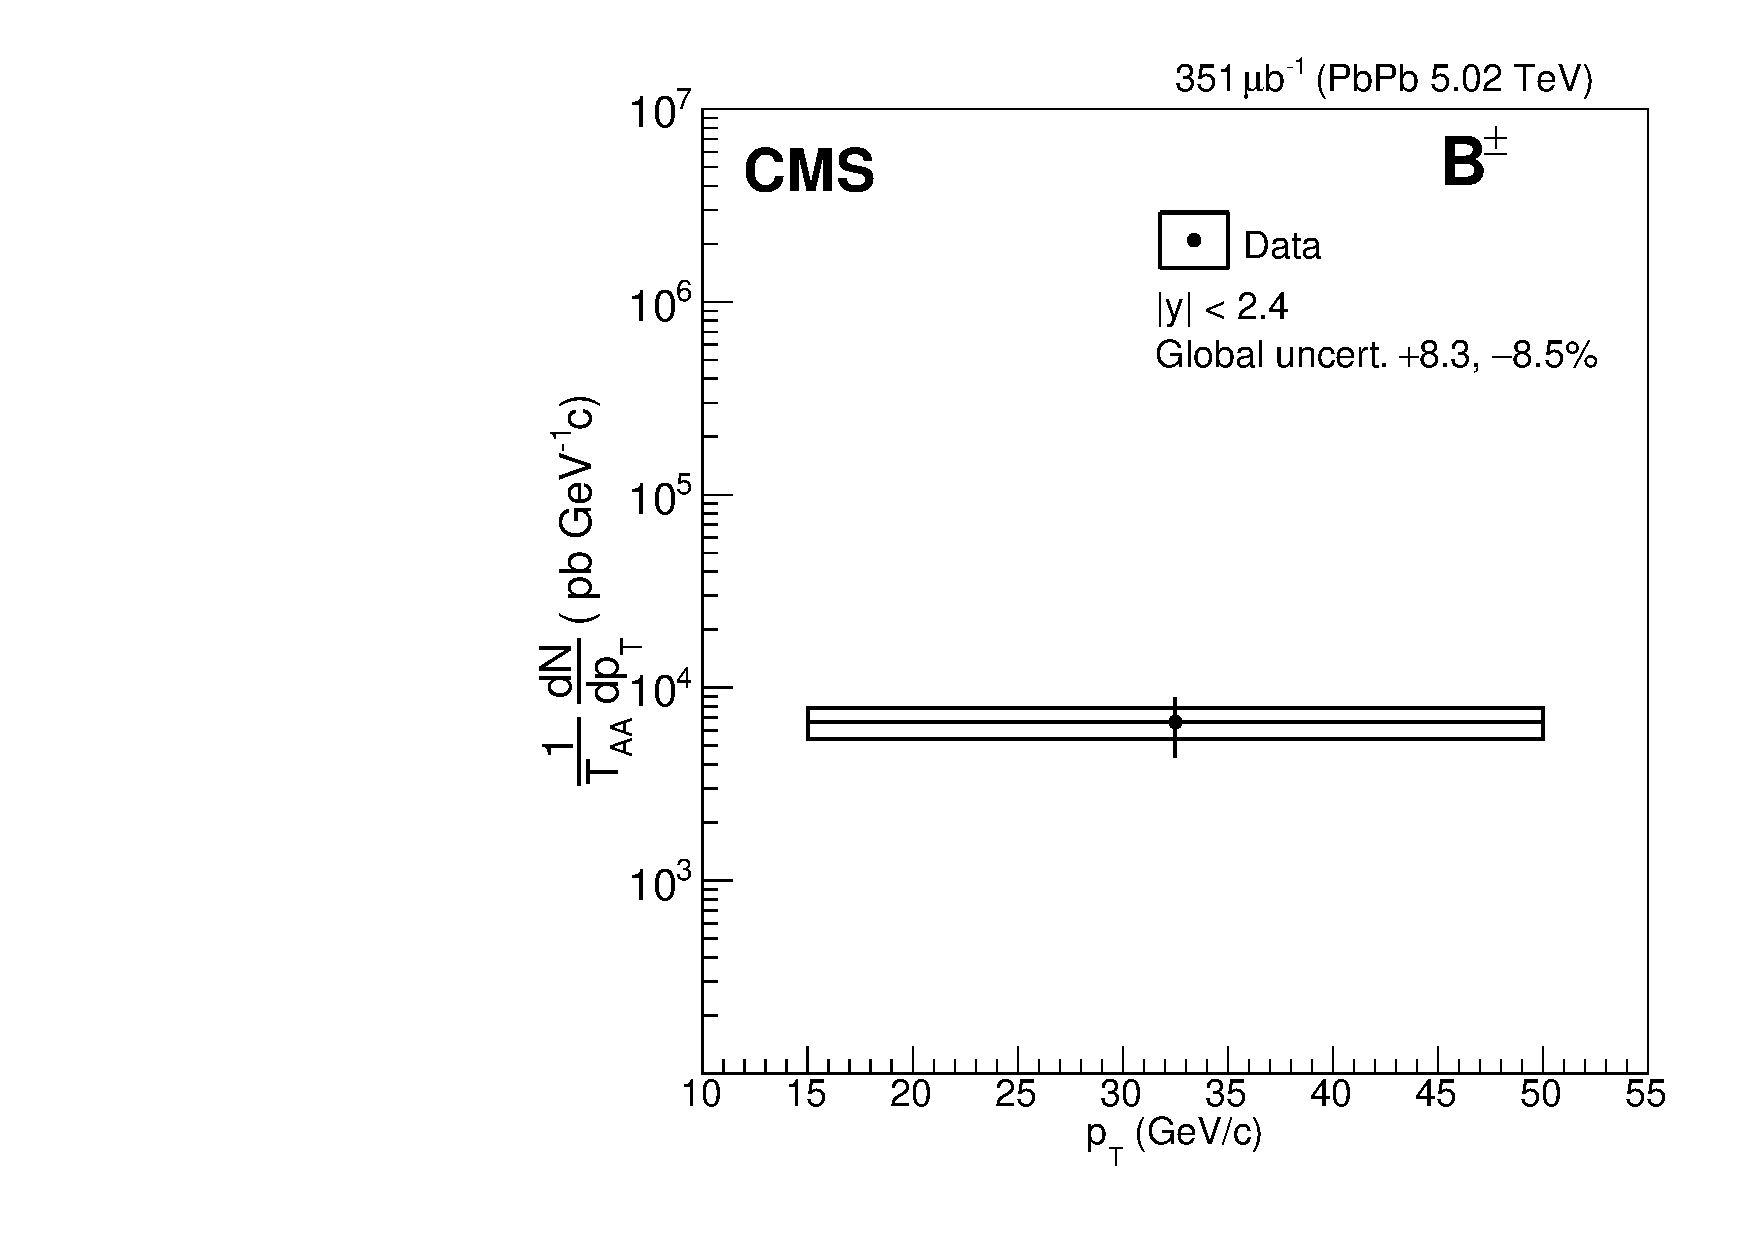
\includegraphics[width=.45\textwidth]{plots/canvasSigmaBplusRatioPbPb_0_100.pdf}
\caption{
The \pt-differential production cross section of $\PBzeros$ in \pp (left) and \PbPb (right) collisions at $\sqrts=5.02\TeV$. The vertical bars (boxes) correspond to statistical (systematic) uncertainties.
The systematic uncertainty boxes here include both the correlated and uncorrelated contributions added in quadrature. The global systematic uncertainty, listed in the legend and not included in the point-to-point uncertainties. 
For the \pp cross section, they comprise the uncertainties in the integrated luminosity measurement and in the branching fraction $\mathcal{B}$. For the \PbPb cross section, they comprise the uncertainties in \TAA, $N_{\text{MB}}$, and $\mathcal{B}$.
The \pp cross section is compared to FONLL calculations~\cite{FONLLcharmbottomPP1,FONLLcharmbottomPP2,FONLLcharmbottomPP3} represented by the colored boxes with the heights indicating the theoretical uncertainty.}
\label{fig:crosssections}
\end{figure*}

 
\begin{figure}[tb]
\centering
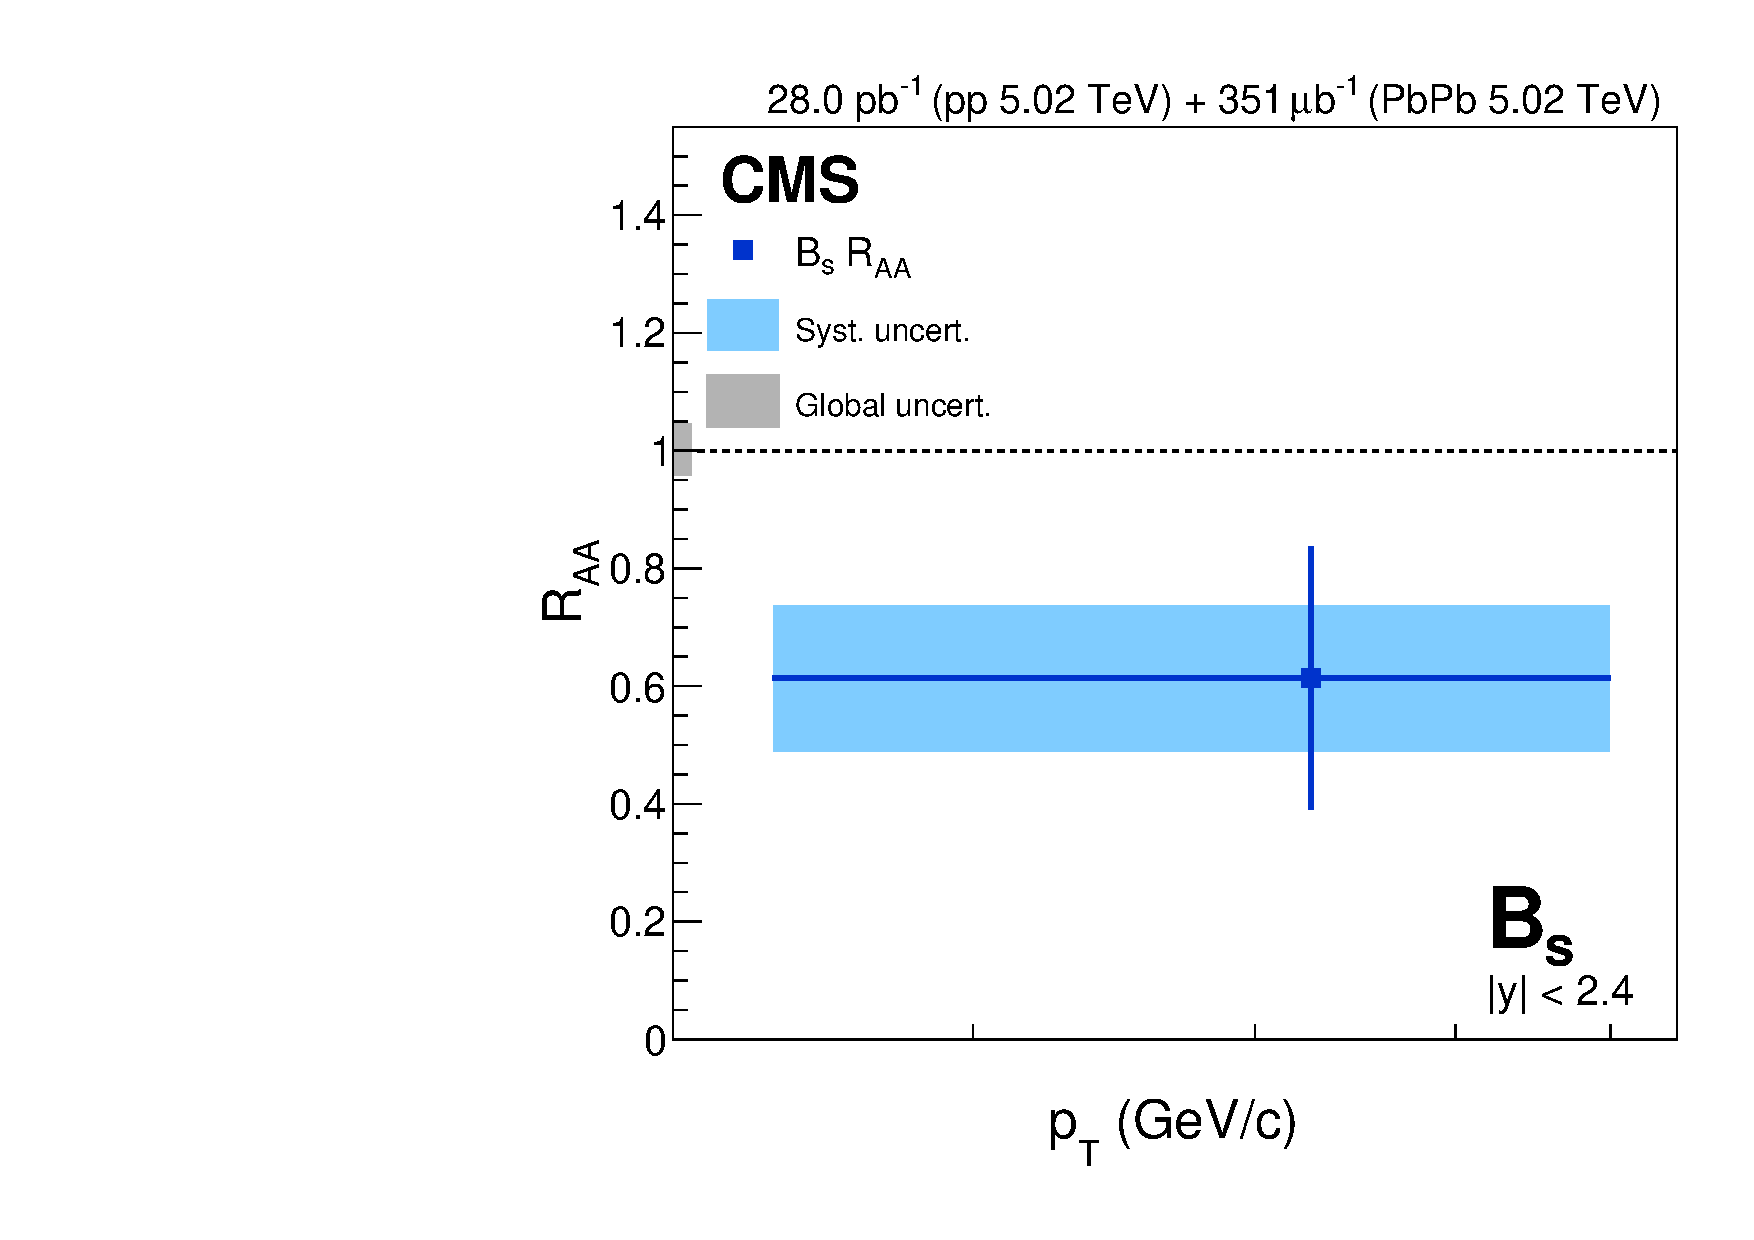
\includegraphics[width=\cmsFigWidth]{plots/canvasRAAPbPb_0_100.pdf}
\caption{The \pt dependence of the nuclear modification factor \RAA of $\PBzeros$ measured in \PbPb collisions at $\sqrtsNN=5.02\TeV$. The vertical bars (boxes) correspond to statistical (systematic) uncertainties.
The global systematic uncertainty, represented as a grey box at $\RAA=1$, comprises the uncertainties in the integrated luminosity measurement and \TAA value. }
%Four theoretical calculations are also shown for comparison: TAMU~\cite{He:2011qa, He:2014cla}, Djordjevic~\cite{Djordjevic:2016vfo}, CUJET3.0~\cite{Xu:2015bbz, Xu:2014tda, Xu:2014ica}, and AdS/CFT HH~\cite{Horowitz:2015dta,  AdscftHH}. The line width of the theoretical calculation from Ref.~\cite{He:2011qa, He:2014cla} represents the size of its statistical uncertainty.}
\label{fig:rpaall}
\end{figure}


\begin{acknowledgments}
We congratulate our colleagues in the CERN accelerator departments for the excellent performance of the LHC and thank the technical and administrative staffs at CERN and at other CMS institutes for their contributions to the success of the CMS effort. In addition, we gratefully acknowledge the computing centers and personnel of the Worldwide LHC Computing Grid for delivering so effectively the computing infrastructure essential to our analyses. Finally, we acknowledge the enduring support for the construction and operation of the LHC and the CMS detector provided by the following funding agencies: BMWFW and FWF (Austria); FNRS and FWO (Belgium); CNPq, CAPES, FAPERJ, and FAPESP (Brazil); MES (Bulgaria); CERN; CAS, MoST, and NSFC (China); COLCIENCIAS (Colombia); MSES and CSF (Croatia); RPF (Cyprus); SENESCYT (Ecuador); MoER, ERC IUT, and ERDF (Estonia); Academy of Finland, MEC, and HIP (Finland); CEA and CNRS/IN2P3 (France); BMBF, DFG, and HGF (Germany); GSRT (Greece); OTKA and NIH (Hungary); DAE and DST (India); IPM (Iran); SFI (Ireland); INFN (Italy); MSIP and NRF (Republic of Korea); LAS (Lithuania); MOE and UM (Malaysia); BUAP, CINVESTAV, CONACYT, LNS, SEP, and UASLP-FAI (Mexico); MBIE (New Zealand); PAEC (Pakistan); MSHE and NSC (Poland); FCT (Portugal); JINR (Dubna); MON, RosAtom, RAS, RFBR and RAEP (Russia); MESTD (Serbia); SEIDI, CPAN, PCTI and FEDER (Spain); Swiss Funding Agencies (Switzerland); MST (Taipei); ThEPCenter, IPST, STAR, and NSTDA (Thailand); TUBITAK and TAEK (Turkey); NASU and SFFR (Ukraine); STFC (United Kingdom); DOE and NSF (USA).
\end{acknowledgments}

\bibliography{auto_generated}



